\documentclass[tikz]{standalone}
% Default preamble
\usepackage{pgfplots}
\pgfplotsset{compat=newest}
\usepgfplotslibrary{groupplots}
\usepgfplotslibrary{polar}
\usepgfplotslibrary{statistics}
\begin{document}
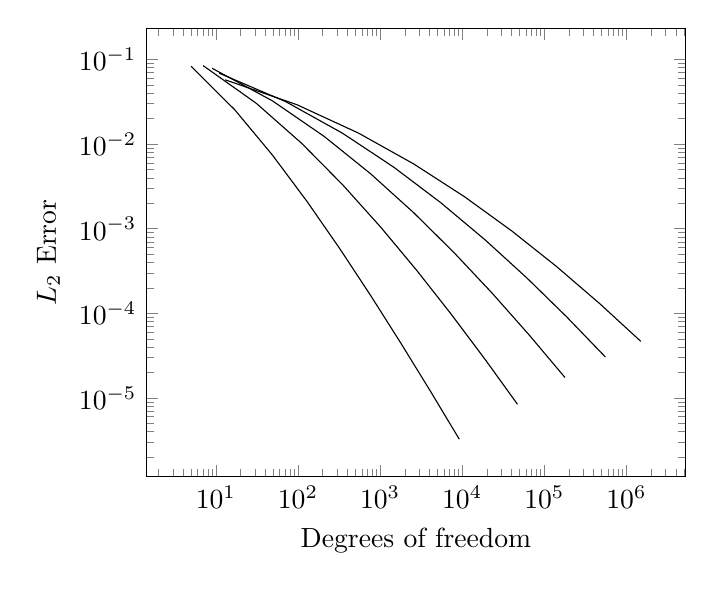
\begin{tikzpicture}[]
\begin{axis}[xlabel={Degrees of freedom}, ylabel={$L_2$ Error}, xmode={log}, ymode={log}]
    \addplot[]
        coordinates {
            (5, 0.08312)
            (17, 0.02547)
            (49, 0.007407)
            (129, 0.002102)
            (321, 0.0005874)
            (769, 0.0001623)
            (1793, 4.442e-5)
            (4097, 1.207e-5)
            (9217, 3.261e-6)
        }
        ;
    \addplot[]
        coordinates {
            (7, 0.08472)
            (31, 0.03044)
            (111, 0.01022)
            (351, 0.003303)
            (1023, 0.001039)
            (2815, 0.0003196)
            (7423, 9.658e-5)
            (18943, 2.873e-5)
            (47103, 8.437e-6)
        }
        ;
    \addplot[]
        coordinates {
            (9, 0.07881)
            (49, 0.03243)
            (209, 0.01232)
            (769, 0.004454)
            (2561, 0.001551)
            (7937, 0.0005236)
            (23297, 0.0001723)
            (65537, 5.545e-5)
            (178177, 1.751e-5)
        }
        ;
    \addplot[]
        coordinates {
            (11, 0.06887)
            (71, 0.03177)
            (351, 0.01341)
            (1471, 0.005334)
            (5503, 0.002027)
            (18943, 0.0007415)
            (61183, 0.0002628)
            (187903, 9.063e-5)
            (553983, 3.053e-5)
        }
        ;
    \addplot[]
        coordinates {
            (13, 0.05755)
            (97, 0.02925)
            (545, 0.01351)
            (2561, 0.005842)
            (10625, 0.002397)
            (40193, 0.0009414)
            (141569, 0.0003564)
            (471041, 0.0001308)
            (1496065, 4.67e-5)
        }
        ;
\end{axis}
\end{tikzpicture}
\end{document}
